% !TeX root = Report.tex

\author{
    Joar Heimonen\\
    \texttt{contact@joar.me}
    \and
    Iselin Skorpen
    \and
    Salim Said
    \and
    Mostafa Mohammadi
    \and
    Ibrar Hussain
    \and
    Hassan Ali Bokhari
}

\documentclass[12pt]{article}
% include enumitem
\usepackage{enumitem}
\usepackage{listings}
\usepackage{sectsty}
\usepackage{color}
\usepackage{float}
\restylefloat{table}
\usepackage{graphicx}
\usepackage{biblatex}

\usepackage{changepage}

\usepackage{xcolor}
\usepackage{listings}

\addbibresource{Library.bib}

\title{\textbf{Group Venus} \\ 4th Delivery: Development Sprint}
\date{\today}

\graphicspath{ {./images/} }

\begin{document}

\subsectionfont{\fontsize{12}{14}\selectfont}

\maketitle

\pagebreak

\tableofcontents



\section{Introduction}
This report aims to document our groups experiences with the groups second design sprint.
We will be covering the topics mentioned above.

\section{Technical background}
This section aims to describe the following terms:
\subsection{Agile development\cite{AgileSoftwareDevelopment2024}}
Agile software development is software that is developed according to the ideas and values presented in the 
Manifesto for Agile Software Development\cite{ManifestoAgileSoftware}.
The manifesto presents the following core ideas:
\begin{itemize}
    \item Individuals and interactions over processes and tools
    \item Working software over comprehensive documentation
    \item Customer collaboration over contract negotiation
    \item Responding to change over following a plan
\end{itemize}
The manifesto is based on ideas created by the Agile Alliance in 2001, 
this is a group of 17 software developers.
\subsubsection{Scrum\cite{Scrum2023}}
Scrum is a type of agile methodology. The methodology was created in 1986 and widely popuralized 
after the manifesto for agile software development was published.
\subsubsection{Scrumwise\cite{scrumwiseScrumToolsScrum}}
Scrumwise is a service for managing a scrumboard. Scrumwise claims it is "The easiest Scrum tool you'll find", 
while this has not been substansiated in any meaningfull way the tool is used by many.
\subsubsection{Scrum master}
The leader of a scrum project is often refered to as the scrum master.
It is the scrum masters task to remove obstacles and streamline the teams development processes.
\subsection{Development sprint\cite{Timeboxing2024}}
A development sprint, also known as a Timebox is the process of allocating a time constraint to
reach a goal. These time constraints usually consists of a week to a month of time.
Timeboxes are great for mitigating risk as per Parkinson's law\cite{ParkinsonLaw2024}
\subsection{Backlog\cite{Backlog2022}}
A backlog usually refers to an accumulation of unfinished work.
\subsection{React\cite{React}}
React is JS\cite{ECMA262} framework for component based development of websites.
\subsubsection{Component based development\cite*{ComponentbasedSoftwareEngineering2024}}
Component based development also known as Component based software engineering is a method of software development
that aims for components of software to be loosely coupled and reusable. Component based development is an 
essential part of any agile workflow.
\subsection{Vite\cite{Vite}}
Vite is a local development server aimed at developing web applications.
\subsection{Pull Request\cite{PullRequests}}
A Pull Request is a proposal to merge one branch with another, usually from different forks of the same repository.
This project heavily relies on pull requests as this allows the scrum master to maintain the intergrity of the project.
\subsection{Burndown graph\cite{BurndownChart2024}}
A burndown graph is a graph that visualizes the remaining tasks in a backlog over time.
This graph is used as a simple status idicator during development sprints.
see \textit{Figure \ref{fig:BD}} for an illustration of a burndown graph.
\subsection{Large Language Models\cite{aiMixtralExperts2023}}
A large language model also known as an LLM is a machine learning model trained on predicting the next word in a series of words.
There are many different LLMs (ChatGTP, Mixtral 7x8b, LLAMA...)
\subsection{Mermaid\cite{MermaidDiagrammingCharting}}
The mermaid desing tool is a diagram and charting tool that was integrated into github in 2022, see \textit{Figure \ref{fig:MM}}.
\begin{figure}[h]
    \begin{verbatim}
    ```mermaid
    graph TD
    A[User] -- Login information --> B{Is Login information valid?}
    B -- Username --> C((DATABASE))
    C -- Hash + Salt --> B
    B -- Valid --> D[JWT-generator]
    B -- Invalid: 500 --> A
    D -- Fetch JWT key --> E(secret_key.txt)
    E -- Key --> D
    D -- Valid JWT --> A
    ```
    \end{verbatim}
    \caption{An example of a mermaid diagram}
    \label{fig:MM}
\end{figure}

\section{Sprint Goal}
The original sprint goal was to start on backend services for the application. This was changed before the sprint started and we decided on using the sprint
to finish off features from the last sprint and document features for the next sprint.

\section{Backlog}
This is the current backlog for the project, see \textit{Figure \ref{fig:BL} and \ref{fig:BL2}}.
\begin{figure}[h]
    \begin{itemize}
        \item Create "Overview" page
        \item Create "Create new" page
        \item Market analysis
        \item Contribution guidelines
        \item Create a text input components for use by other components
        \item Make the grid re-arrange when there is not enough space left
        \item Setup react router
        \item Create a Login/user page
        \item Password strength checker
    \end{itemize}
    \caption{Our backlog}
    \label{fig:BL}
\end{figure}
\begin{figure}[h]
    \begin{adjustwidth}{-1in}{-1in}
        \centering
        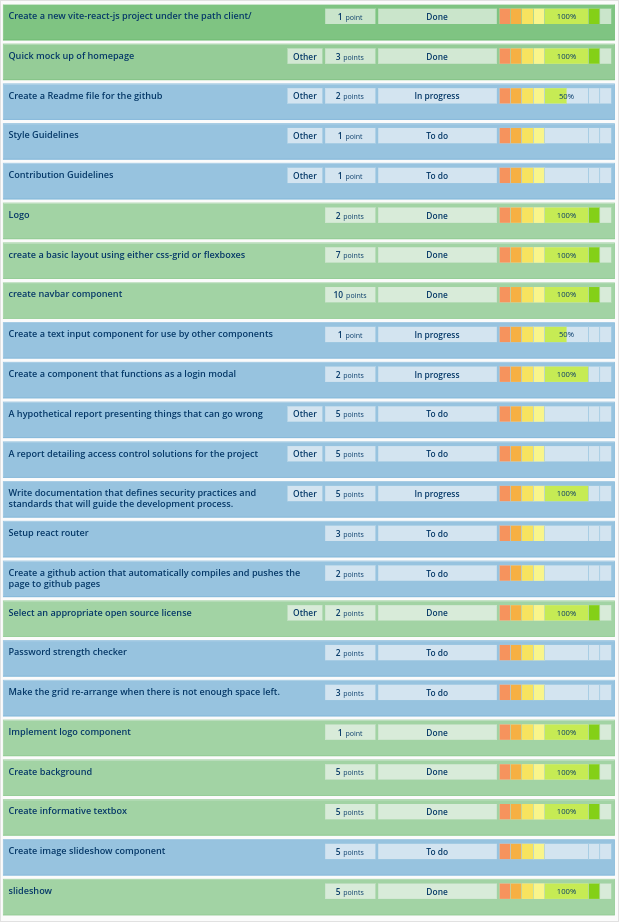
\includegraphics[scale=0.5]{backlog.png}
        \caption{An image of a scrumwise backlog}
        \label{fig:BL2}
    \end{adjustwidth}
\end{figure}
\clearpage

\section{Time}
\subsection{Participation}
This is information taken from the "Time used in this sprint" page on scrumwise.
\subsubsection{Joar Heimonen}
Joar Heimonen is the scrum master of this project. Heimonen implemented a document outlinining the architecture related to access control:
\url{https://github.com/Slenderman00/show-it/blob/main/docs/access-control.md}
Heimonen also implemented the following:
    \begin{itemize}
        \item Add logo.
        \item Create a Readme file for the github.
        \item Create image slideshow component.
        \item A report detailing access control solutions for the project. \cite{ShowitDocsAccesscontrol}
        \item Create a github action that automatically compiles and deploys the page.
        \item Navbar - The navbar should show what page the user has selected.
        \item Create "Create new" page.
        \item Create "overview" page.
        \item Style navbar.
    \end{itemize}
It is worth mentioning that Heimonen was abscent two days during this sprint due to surgery.
This does not seem to have caused any notable obstructions for the team.

\subsubsection{Iselin Skorpen}
Iseling skorpen finished up and formalized the design of the application this sprint. This resulted in the following document:
\url{https://github.com/Slenderman00/show-it/blob/main/docs/visual-design.md}
    \begin{itemize}
        \item Design and mock up "overview" page.
        \item Design and mock up "Create new" page.
        \item Document showing and describing design mockups. \cite{ShowitDocsVisualdesign}
        \item Put together a homepage
    \end{itemize}
\subsubsection{Salim Said}
Salim Said did not contribute.
\subsubsection{Mostafa Mohammadi}
Mostafa Mohammadi did not contribute.
\subsubsection{Ibrar Hussain}
Ibrar Hussain did not contribute.
\subsubsection{Hassan Ali Bokhari}
Hassan Ali Bokhari did not contribute.

\subsection{Time list}

For a picture of our time list see \textit{Figure \ref{fig:TL}}. During this sprint we only had a meeting that lasted an hour, this consisted mainly of sprint planning and a sprint retrospective.
Due to the large ammount of time spent in meetings during the last sprint the team had a cohesive idea of what had to be done.
\begin{figure}[h]
    \begin{adjustwidth}{-1in}{-1in}
        \centering
        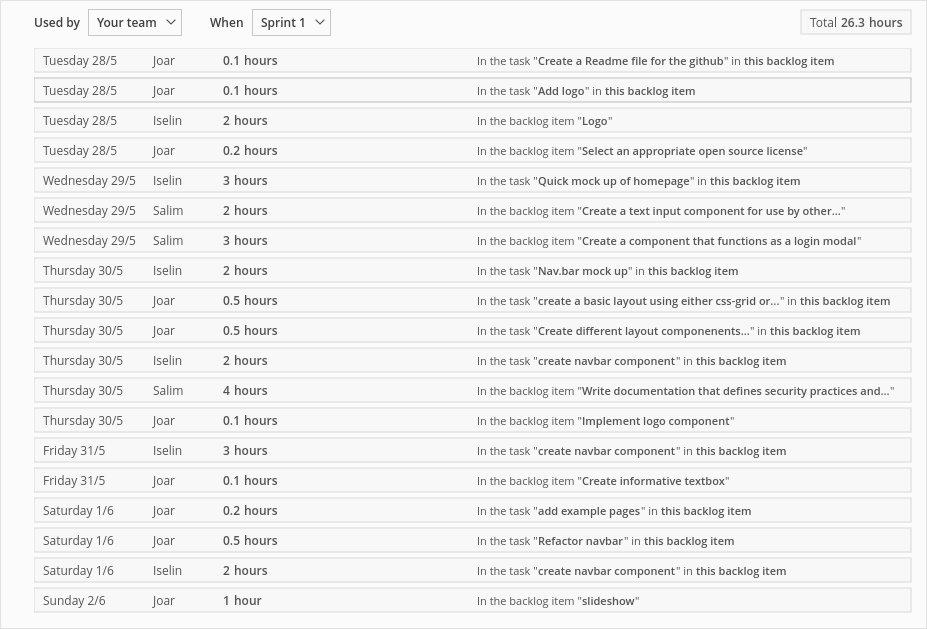
\includegraphics[scale=0.5]{timelist.png}
        \caption{An image of a scrumwise time list}
        \label{fig:TL}
    \end{adjustwidth}
\end{figure}
\clearpage
% insert picture of burndwn graph
\subsection{Burndown graph}
During our first sprint our burndown graph flattened out due to the scope of the sprint growing. This time we tried to avoid adding tasks to the sprint, this resulted in the following burndown graph as seen in
\textit{Figure \ref{fig:BD}}.
\begin{figure}[h]
    \begin{adjustwidth}{-1in}{-1in}
        \centering
        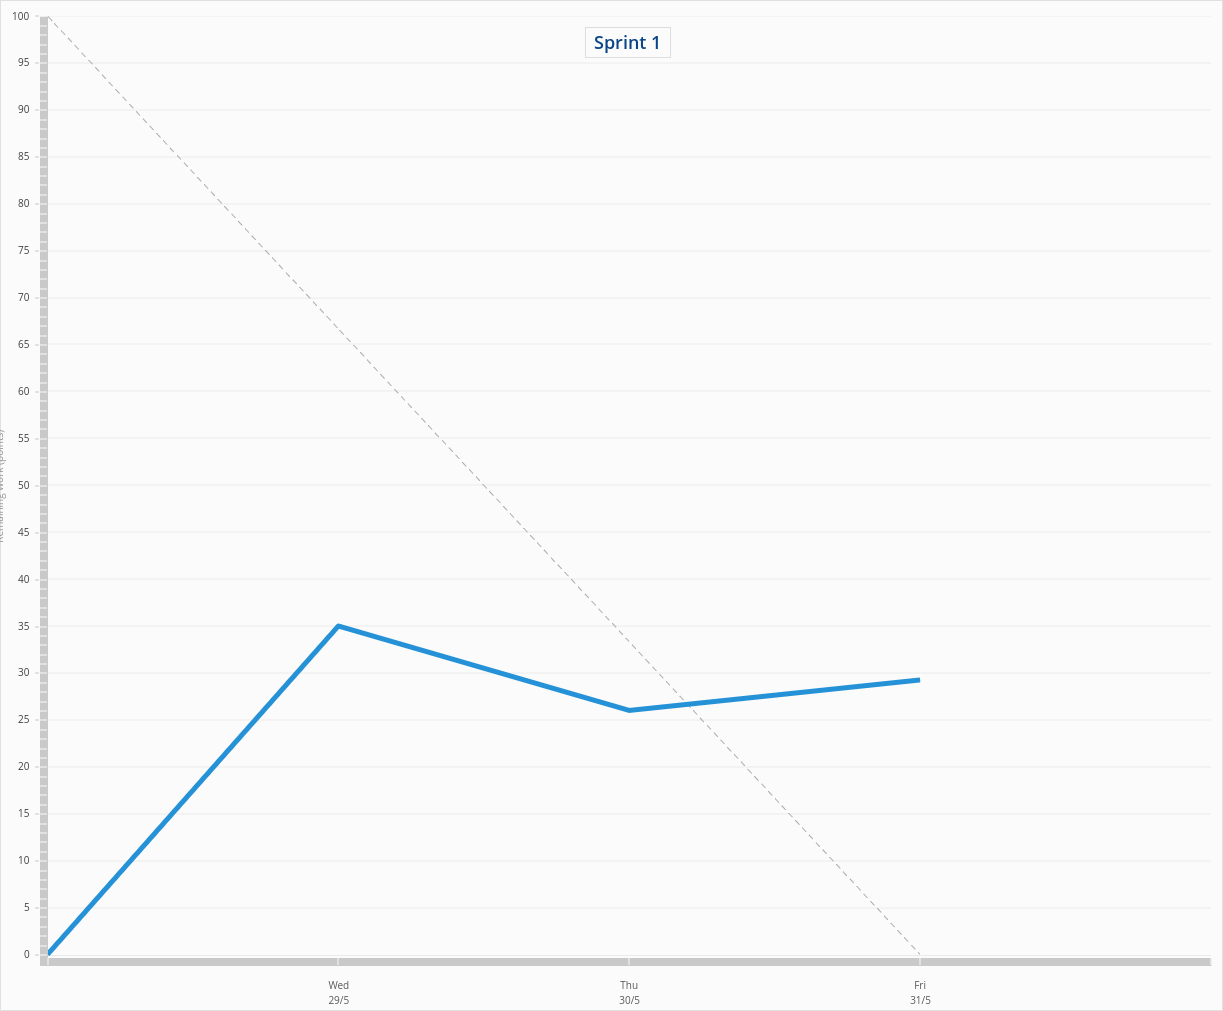
\includegraphics[scale=0.4]{burndown.png}
        \caption{An image of a scrumwise burndown graph}
        \label{fig:BD}
    \end{adjustwidth}
\end{figure}
\clearpage

\section{Usage of Large Language Models}
During this sprint, different LLMs have been used, one of the more utilized LLMs is the mixtral 7x8b model created by Mistral AI 
\cite{aiMixtralExperts2023}. For inference on this model, we have been using a tool known as 
\textbf{Ask-Surf} \cite{heimonenSlenderman00AskSurf2024}. Ask-surf allows users to interact with an LLM 
like any other Unix application, thus allowing for syntax like this: \begin{verbatim} "dig https://joar.me | surf explain this data to me" \end{verbatim}
and this:
\begin{verbatim} "component.jsx > surf why does this component not render" \end{verbatim}
Our software is open-source, but when developing proprietary software, it is especially important to consider what kind of third-party services you are exposing your clients' intellectual property to.
\\
\\
One of Surfs main use cases has been to suggest topics for different reports and tasks for the team, as the majority of the team
are cybersecurty students.

\section{Reflection}
This section will anwser the following questions:
\begin{itemize}
    \item Could you have done anything differently?
    \item What were you particularly satisfied with?
\end{itemize}

\subsection{Could you have done anything differently?}
We have been extremely relaxed when it comes to group memebers not showing up and not participating, while 
we do not quite know how to deal with this it is aboslutely something that should have been dealt with differently.
As the results have been disappointing.

\subsection{What were you particularly satisfied with?}
While we did not manage to achieve our goals we spent a lot of time thinking of more theoretical and practical aspects of our application.
This resulted in some beautiful designs by Iselin Skorpen \url{https://github.com/Slenderman00/show-it/blob/main/docs/visual-design.md}.
We are also especially satisfied with the access control document (\url{https://github.com/Slenderman00/show-it/blob/main/docs/access-control.md})
as it features lots of beautiful graphs created using \textbf{Mermaid}\cite{MermaidDiagrammingCharting}


\section{Heimonens Notes}
Group participation during this sprint has been even lower than the last sprint. Certain group members
have been offering to help but when given the opportunity they have gone offline. We tried giving the more inactive group memebers
free reigns during this sprint but this had little to no effect. We currently find ourself at a loss, there does not seem to be any way
of inspiring these group members to contribute, even with no restrictions on contributions they are still abscent.
\\
\\
Due to low group participation we have taken the unilateral decision to shift the focus of our last 
sprint to finishing creating a working prototype of the frontend of the application. The offer still stands for
group members to contribute with whatever they want as long as it is not directly harmfull to the health of the codebase.

\pagebreak
\printbibliography

\end{document}